\documentclass[a4paper,12pt]{extreport}
\usepackage[utf8]{inputenc}
\usepackage[russian]{babel}
\usepackage{ragged2e}
\usepackage[mag=1000,a4paper,left=1cm,right=1cm,top=1cm,bottom=1cm,noheadfoot]{geometry}
\usepackage{mathtext}
\usepackage{amsmath,amssymb,amsthm,amscd,amsfonts,graphicx,epsfig,textcomp,wrapfig}
\usepackage[dvips]{graphicx}
\graphicspath{{noiseimages/}}

\newcommand{\tab}{\hspace{10mm}}
\newcommand{\name}{
			\normalsize
			{
				\ \ \quad
                \mbox{} \hfil {\flushleft{взлет}} \hfill {22.01.2024}
			%\quad
			}
			\vspace{5pt}\hrule
		}

\def\head#1#2{
	\begin{center}{
			\LARGE
			\bf #2
			
			{\normalsize \bf #1}
			\vspace{-10pt}
	}\end{center}
}

\newcommand{\del}{\mathop{\raisebox{-2pt}{\vdots}}}
\newcommand{\q}{}

\newcounter{tasknum}
\setcounter{tasknum}{0}
\def\thetasknum{{\textbf{\arabic{tasknum}}}}
\newcommand{\task}{\refstepcounter{tasknum}\vspace{2pt}\noindent \textbf{} \thetasknum\textbf{.}~}
\newcommand{\coff}{\refstepcounter{tasknum}\vspace{2pt}\noindent \textbf{Задача} \thetasknum *\textbf{.}~}


\newcommand{\eq}[1]{\underset{#1}{\equiv}}
\newcommand{\dv}{\ensuremath{\mathop{\raisebox{-2pt}{\vdots}}}}
\newcommand{\ndv}{\not \dv}

\newcounter{exnum}
\setcounter{exnum}{0}
\def\theexnum{{\emph{\arabic{exnum}}}}
\newcommand{\ex}{\refstepcounter{exnum}\vspace{2pt}\noindent \emph{Упражнение} \theexnum\emph{.}~}



\theoremstyle{plain}
\newtheorem{theorem}{Теорема}
\newtheorem{lemma}{Лемма}
\newtheorem{proposition}{Предложение}
\newtheorem{corollary}{Следствие}
\theoremstyle{definition}
\newtheorem{definition}{Определение}
\theoremstyle{remark}
\newtheorem{remark}{Замечание}
\newtheorem{example}{Пример}

\textheight=250mm %
\textwidth=180mm %
\oddsidemargin=-10.4mm%
\evensidemargin=-10.4mm %
\topmargin=-24.4mm


\begin{document}
	\pagestyle{empty}
    \name{}
	\head{группа 9.1}{ТЧ}
	\bigskip
	
\task Целые числа $a, b$ и $c$ таковы, что $a^3 + b^3 + c^3$ делится на $7$. Докажите, что $abc$ делится на $7$.\\

\task  У двух натуральных чисел сложили сумму и произведение. Могло ли получитсья $100$?\\

\task Найдите все такие целые $a$ и $b$, что $3ab+b-5a=45$.\\

\task Докажите, что найдутся $2024$ последовательных числа, таких, что $k$-ое по счету число делится на $p_{k}^{3}$, где $p_{k}$ - $k$-ое по счету простое число.\\

\task Множество $S$ состоит из чисел $1, 1+b, 1+b+b^2, ...$, где $b$ — некоторое натуральное число. Докажите, что если два числа из $S$ являются членами возрастающей арифметической прогрессии, то найдётся ещё одно число из $S$, также являющееся членом этой прогрессии.\\

\task Найдите все такие тройки натуральных чисел, что произведение любых двух даёт остаток $1$ при делении на третье.
\\

\task  Занумеруем все простые числа в порядке возрастания: $p_1 = 2, p_2 = 3, \dots $ Может ли среднее арифметическое $\frac{p_1+...+p_n}{n}$ при каком-нибудь $n \geq 2$ быть простым числом?\\

\task Докажите, что в любой арифметической прогрессии составленной из натуральных чисел, есть бесконечно много членов, в разложении которых на простые множители входят в точности одни и те же простые числа.\\

\task Каждое ли целое число можно записать как сумму кубов нескольких целых чисел, среди которых нет одинаковых?
\\

 \begin{center}
  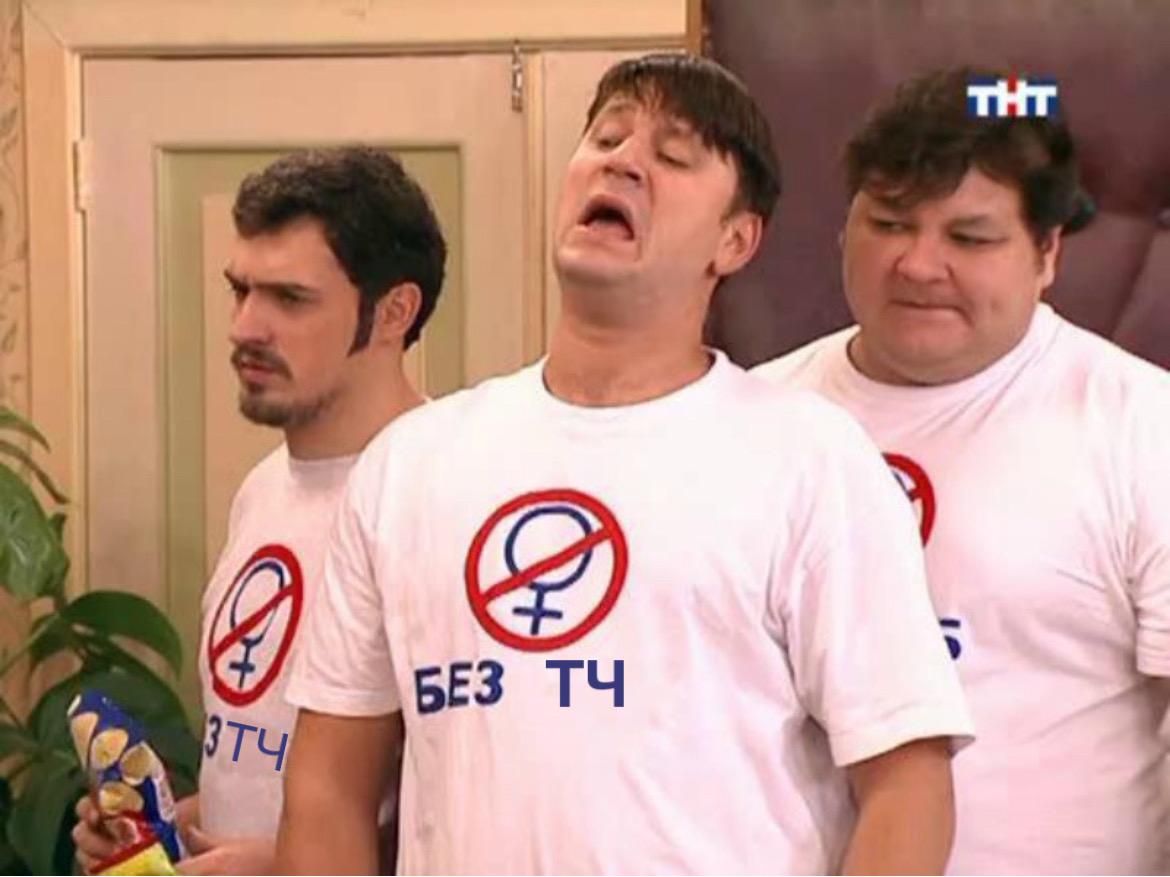
\includegraphics[width=0.4\textwidth]{bb.JPEG}
  \end{center} 

\end{document}
